\documentclass[11pt, oneside]{article}   	% use "amsart" instead of "article" for AMSLaTeX format
\usepackage{geometry}                		% See geometry.pdf to learn the layout options. There are lots.
\geometry{letterpaper}                   		% ... or a4paper or a5paper or ... 
%\geometry{landscape}                		% Activate for for rotated page geometry
%\usepackage[parfill]{parskip}    		% Activate to begin paragraphs with an empty line rather than an indent
\usepackage{graphicx}				% Use pdf, png, jpg, or eps§ with pdflatex; use eps in DVI mode
								% TeX will automatically convert eps --> pdf in pdflatex		
\usepackage{amssymb}
\usepackage{amsmath}
\usepackage{parskip}
\usepackage{color}
\usepackage{hyperref}

\title{Inverse and integer powers}
%\author{The Author}
%\section{}
%\subsection*{}
\date{}							% Activate to display a given date or no date

\graphicspath{{/Users/telliott_admin/Dropbox/Tex/png/}}
% \begin{center} 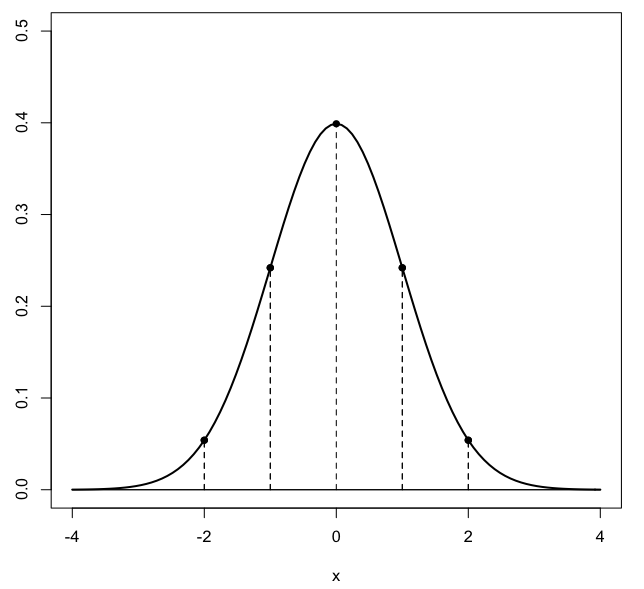
\includegraphics [scale=0.4] {gauss3.png} \end{center}
\begin{document}
\maketitle
\Large
\subsection*{square}
Consider 
\[ f(z) = z^2 \]
\[ = (x + iy)(x + iy) \]
\[ = x^2 - y^2 + i2xy \]
\[ u(x,y) = x^2 - y^2 \]
\[ v(x,y) = 2xy \]
Note that
\[ u_x = 2x = v_y \]
\[ u_y = -2y = - v_x \]
The Cauchy-Riemann conditions (CRE) hold.

Compute the derivative as follows:
\[ \frac{df}{dz} = u_x + i v_x \]
\[ = 2x + i 2y = 2z \]
or alternatively
\[ \frac{df}{dz} = v_y - i u_y \]
\[ = 2x - i (-2y) = 2x + i2y = 2z \]

This is the result we would expect to get by simply differentiating f(z) as if it was a real function. For analytic functions this will always be the case.

\subsection*{cube}
Let
\[ f(z) = z^3 = (x + iy)^3 \]
\[ = (x + iy)(x^2 - y^2 + i2xy) \]
\[ = x^3 -xy^2 + i2x^2y + ix^2y -iy^3 - 2xy^2 \]
\[ = x^3 - 3xy^2 + i(3x^2y - y^3) \]
So
\[ u(x,y) = x^3 - 3xy^2 \]
\[ v(x,y) = 3x^2y - y^3 \]
and
\[ u_x = 3x^2 - 3y^2 \]
\[ v_x = 6xy \]
That means
\[ \frac{df}{dz} = u_x + i v_x \]
\[ = 3x^2 - 3y^2 + i 6xy \]
\[ = 3 \ [ x^2 - y^2 + i2xy \ ] \]
\[ = 3z^2 \]

We could continue and show that $z^n$ is analytic for any positive integer power of $n$.
Notice the pattern for $i$:
\[ (x + iy)^n = x^n + nx^{n-1}(iy) + (n)(n-1)x^{n-2}(iy)^2 + \dots \]
The progression goes:
\[ i^0, i^1, i^2, i^3 \]
\[ = 1, i, -1, -i \]
and then repeats.

\subsection*{inverse}
Using the complex conjugate is a good way to work with the inverse function (or with division by any complex number):
\[ \frac{1}{z} = \frac{z*}{zz*} = \frac{x - iy}{x^2 + y^2} \]
or in polar notation:
\[  \frac{1}{z} =  \frac{r e^{-i \theta}}{r^2 \ e^{i \theta} \ e^{-i \theta}} = \frac{1}{r} \ e^{-i \theta} \]

Let's look at what it means to take the inverse for different $z$.  In every case, the point is reflected across the $x$-axis (the ray makes an angle $- \theta$ with the $x$-axis).  

There is no change in length for $r=1$.  But if say 
\[ z = 1 + i = (1,1) = \sqrt{2} \ e^{i \cdot \pi/4} \]
then the new point has $r = \frac{1}{\sqrt{2}}$ and it is located at
\[ \frac{1}{z} = \frac{1}{\sqrt{2}} e^{-i \cdot \pi/4} = (\frac{1}{2},- \frac{1}{2}) = \frac{1}{2} - i \frac{1}{2}\]

Differentiate
\[ f(z) = 1/z \]
\[ = \frac{z*}{zz*} \]
\[ = \frac{x}{x^2 + y^2} - i\frac{y}{x^2 + y^2} \]
Now let's do the partial derivatives.  $u(x,y)$ has $x$ in both the numerator and the denominator.

Recall the quotient rule (reusing the symbols $g$ and $h$):
\[ (g/h)' = (g'h - gh')/h^2 \]

So:
\[ u_x = \frac{1}{(x^2 + y^2)^2} \ (x^2 + y^2 - 2x^2) \]
\[ = \frac{y^2 - x^2}{(x^2 + y^2)^2} \]
To do $v_y$ just switch $x$ and $y$ in the result, but remember to then multiply by the leading factor of $-1$:
\[ v_y = (-1) \ \frac{x^2 - y^2}{(x^2 + y^2)^2} = \frac{y^2 - x^2}{(x^2 + y^2)^2} \]
Thus $u_x = v_y$

Now for the other ones we have that
\[ u(x,y) = \frac{x}{x^2 + y^2} \]
which only involves $y$ in the denominator so the derivative is just
\[ u_y = x \ \frac{1}{(x^2 + y^2)^2} \ (-1) (2y) \]
\[ = \frac{-2xy}{(x^2 + y^2)^2} \]
For $v_x$ we have 
\[ v(x,y) = \frac{-y}{x^2 + y^2} \]
Again, we have $x$ only in the denominator so the derivative is
\[ (-y) \ \frac{1}{(x^2 + y^2)^2} \ (-1) (2x) \]
\[ = \frac{2xy}{(x^2 + y^2)^2} \]
We see that $u_y = - v_x$.

So the CRE are satisfied (except at $z=0$) and the derivative is
\[ \frac{df}{dz} = u_x + i v_x \]
\[ =  \frac{y^2 - x^2}{(x^2 + y^2)^2} + i \frac{2xy}{(x^2 + y^2)^2} \]
\[ = \frac{1}{(x^2 + y^2)^2} \ (y^2 - x^2 + i2xy) \]
We expect that this should be (in disguise) $-1/z^2$.  Let's see:
\[ \frac{1}{z} =  \frac{z*}{zz*} \]
\[ \frac{1}{z^2} =  \frac{(z*)^2}{(zz*)^2} \]
The denominator is certainly correct since
\[ zz* = x^2 + y^2 \]
What about
\[ (z*)^2 = (x - iy)(x - iy) = x^2 - y^2 - i2xy \]
so
\[ -(z*)^2 = (-1)(x - iy)(x - iy) = y^2 - x^2 + i2xy \]
Everything checks.

\subsection*{powers:  de Moivre's formula}
Let $n$ be an integer:
\[ z^n = (re^{i\theta})^n = r^n e^{in\theta} \]
Suppose $r=1$:
\[ z^n = e^{in\theta} = \cos n \theta + i \sin n \theta \]
\[ (\cos \theta + i \sin \theta)^n = \cos n \theta + i \sin n \theta \]
This is de Moivre's formula.

Suppose $n=2$, then
\[ (\cos \theta + i \sin \theta)^2 \]
\[ = \cos^2 \theta - \sin^2 \theta + i\ 2 \sin \theta \cos \theta \]
Equating with the right-hand side of de Moivre's formula:
\[ \cos^2 \theta - \sin^2 \theta + i\ 2 \sin \theta \cos \theta = \cos 2 \theta + i \sin 2 \theta \]
we find that
\[ \cos 2 \theta = \cos^2 \theta - \sin^2 \theta \]
\[ \sin 2 \theta = 2 \sin \theta \cos \theta \]
We already know these, they are the double angle formulas.

Suppose $n=3$, then
\[ (\cos \theta + i \sin \theta)^3 \]
\[ = \cos^3 \theta - 3 \cos \theta \sin^2 \theta + i (3 \cos^2 \theta \sin \theta - \sin^3 \theta) \]
we find that
\[ \cos 3 \theta =\cos^3 \theta - 3 \cos \theta \sin^2 \theta \]
\[ \sin 3 \theta = 3 \cos^2 \theta \sin \theta - \sin^3 \theta \]
and so on.

We can just check that last one for $\theta = \pi/6$:
\[ \sin 3 \theta = 3 \cos^2 \theta \sin \theta - \sin^3 \theta \]
\[ 1 = 3 (\frac{\sqrt{3}}{2})^2 \ \frac{1}{2} - (\frac{1}{2})^3 \]
Multiply both sides by $2^3$:
\[ 8 = 3 (\sqrt{3})^2 - 1 \]
That looks correct.

\end{document} 